% 6. Results
%   6.1. Anatomical
%   6.2. Mechanical Simulation
\section{Results}
\label{sec:results}

% - Disegno surrogato anatomico dell'albero respiratorio.  (output da
%   ParaView).
% - Grafici: un gradino "sopra" (10) le soglie e uno "sotto" (8) (xlims
%   = (.995, 1.09)).

% Grafici dipendenti dal numero di generazioni (?)

\subsection{Anatomical}
\label{subsec:anatomical_results}

% AGGIUNTA MODIFICA, COMPLETARE
% {\color{red} Completare XX facendo simulazioni}

A CT of a 40-week infant was collected. We segmented and extracted the
centreline of 19 major airways, down to 5$^{\text{th}}$ generation.
We also obtained four lobes.

% Mostra immagine delle vie aeree segmentate (skeletonizzazione della
% centreline) e dei quattro lobi su tre piani (xy, xz, yz).

\begin{figure}[H]\centering
  \subfloat[][x-y plane]{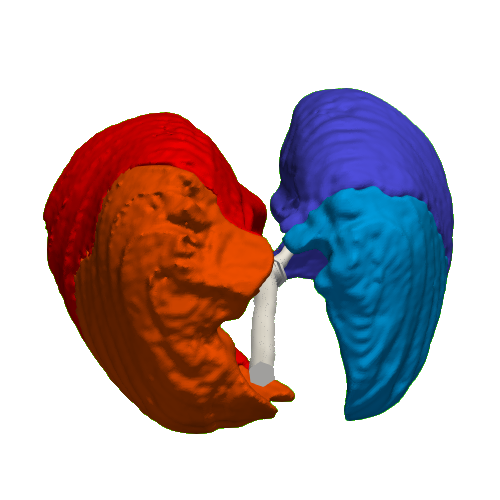
\includegraphics[width=.45\textwidth]{major_airways_xy.png}}%
  \hspace{1cm}
  \subfloat[][y-z plane]{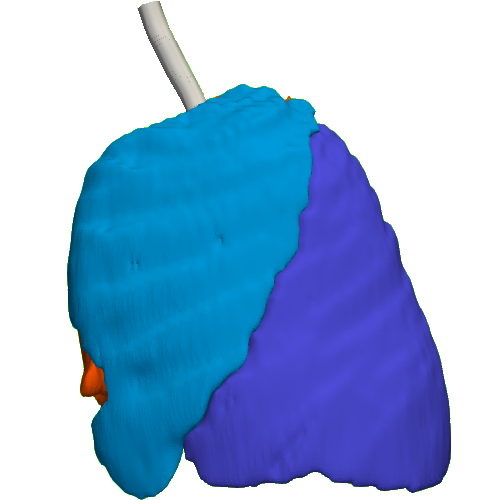
\includegraphics[width=.45\textwidth]{major_airways_yz.png}}\\\vspace{1cm}
  \subfloat[][x-z plane]{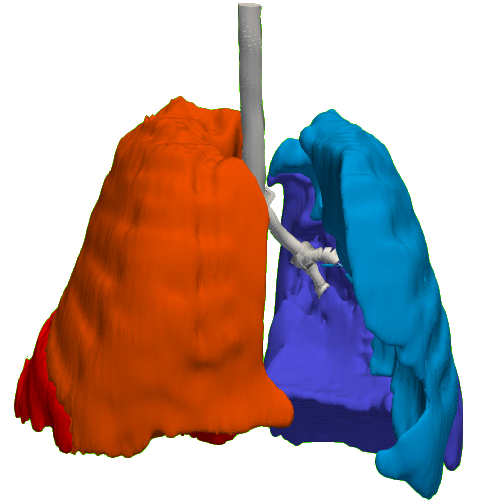
\includegraphics[width=.45\textwidth]{major_airways_xz.png}}

  \caption{Major Airways and Lobes segmentations.  Cyan: Upper Left
    Lung; Blue: Lower Left Lung; Orange: Upper Right Lung; Red: Lower
    Right Lung.}
  \label{fig:anatomical_results}
\end{figure}

Using the developed program, based on the Lung Chaste library, we
reconstructed the missing generations starting from 15000 seed points
per lung.  The obtained airway tree can be displayed by ParaView.
% Mostra immagine dell'albero completo.

\begin{figure}[H]\centering
  \subfloat[][x-y plane]{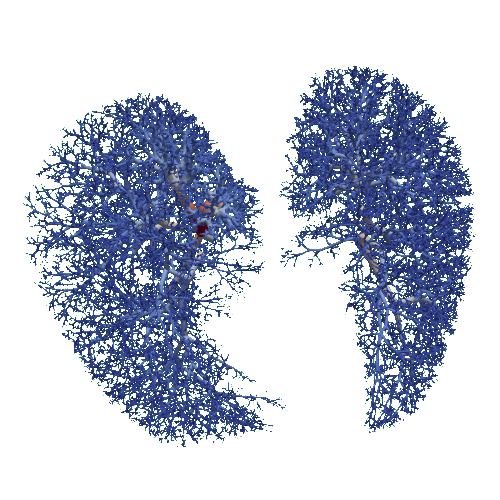
\includegraphics[width=.45\textwidth]{complete_airways_xy.png}}%
  \hspace{1cm}
  \subfloat[][y-z plane]{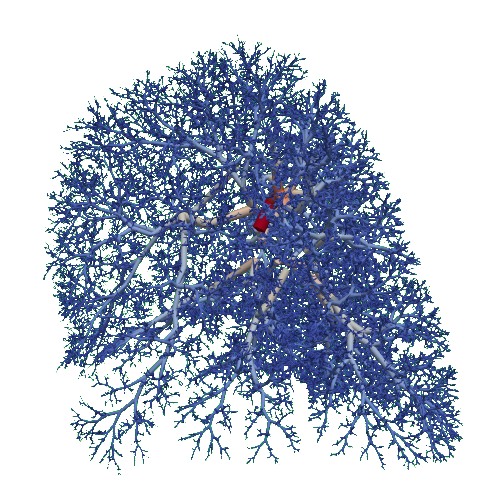
\includegraphics[width=.45\textwidth]{complete_airways_yz.png}}\\\vspace{1cm}
  \subfloat[][x-z plane]{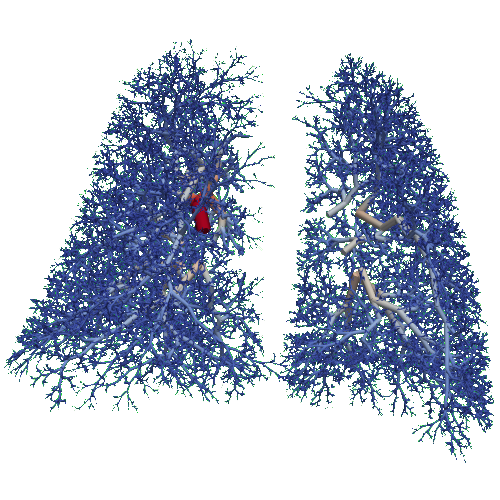
\includegraphics[width=.45\textwidth]{complete_airways_xz.png}}

  \caption{Complete Airways generated by Chaste User Project (major
    airways are here excluded).  They are color-coded with respect to
    their radii.}
  \label{fig:complete_anatomical_results}
\end{figure}

The lobes are fully covered by the statistically generated airways and
this allows us to move a step forward in newborn lung simulation.

\subsection{Mechanical Simulation}
\label{subsec:mechanical_results_subsec}

% Descrizione dei test.  La descrizione della rete in termini di
% parametri va fatta qui?

% Introduzione da aggiungere: lo scopo di queste simulazioni. Queste non
% sono le simulazioni per capire come va il bambino ma per verificare la
% coerenza dei comportamenti dei vari componenti.  Facendo riferimento
% alla figura della sottorete che ho considerato.  Nella sottorete
% abbiamo applicato due livelli diversi di pressione: una sopra la
% pressione capillare, così da aprire tutti i diodi dei vari moduli e
% una sotto la pressione capillare di qualche diodo per vedere le
% differenze.

These simulations are to verify the various components and modules
coherence.  Two tests have been designed as follows.  A step voltage
generator is applied to the electrical equivalent of the newborn lung.
The step amplitude is 10V for the first test and 8V for the second.
In both tests, the step voltage is applied at $t=1$s from the start of
the simulation.

The reason why these values for voltage have been chosen is related
both to the airway subtree described in \Cref{fig:subtree_development}
and to the diode threshold values ``vin\_th'' for airways and acini in
\Cref{tab:airways_test1,tab:acini_test1,tab:airways_test2,tab:acini_test2}.

% Faccio una descrizione di queste curve: si aprono le vie aeree dalla
% più vicina a quella più lontana e gli acini seguono un determinato
% ordine di apertura.

% Quando cambio soglia abbiamo notato che alcuni acini non si aprono
% in quanto la pressione capillare è troppo elevata.  Il fatto di aver
% abbassato la pressione ha rallentato l'apertura di tutti quanti perché
% ci mettono un po' a raggiungere la pressione capillare.  Cambia la
% sequenza di apertura degli acini.  Posso usare nella descrizione dei
% grafici anche i nomi IAE, IAI ecc (facendo però riferimento al
% capitolo in cui introduco il problema).

% AGGIUNTA MODIFICA, COMPLETARE
% To verify the behavior of the mechanical components
% implemented in Julia, we tested the system described by applying

The first test employs a step amplitude for the voltage generator which
overcomes every module diode threshold.  It is possible to check out in
\Cref{fig:mechanical_results_10_1,fig:mechanical_results_8_1} modules
opening times and activation orders.  Airways open from the most
proximal to the most distal one.  It is more interesting to analyze
the activation order of the acini.  They open following a proximal
to distal order but high diode thresholds introduce delays.

% Inserisco gli output di Julia, in particolare correnti e tensioni
% sotto e sopra threshold. (ampiezza scalino di 8 e 10V).
\vspace{2.25em}

\begin{figure}[H]\centering
  \subfloat[][Airways voltages]{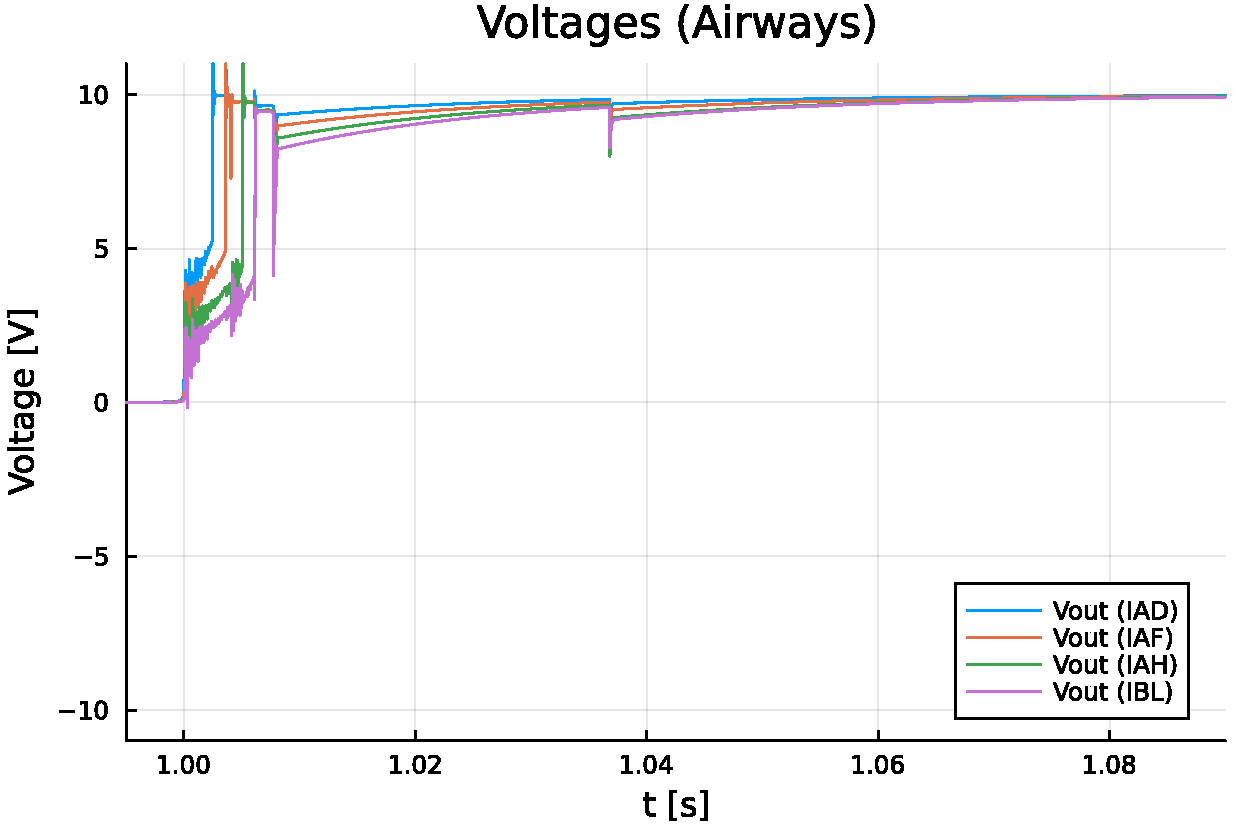
\includegraphics[width=.45\textwidth]{airways_voltages_10.pdf}}%
  \hspace{1cm}
  \subfloat[][Airways currents]{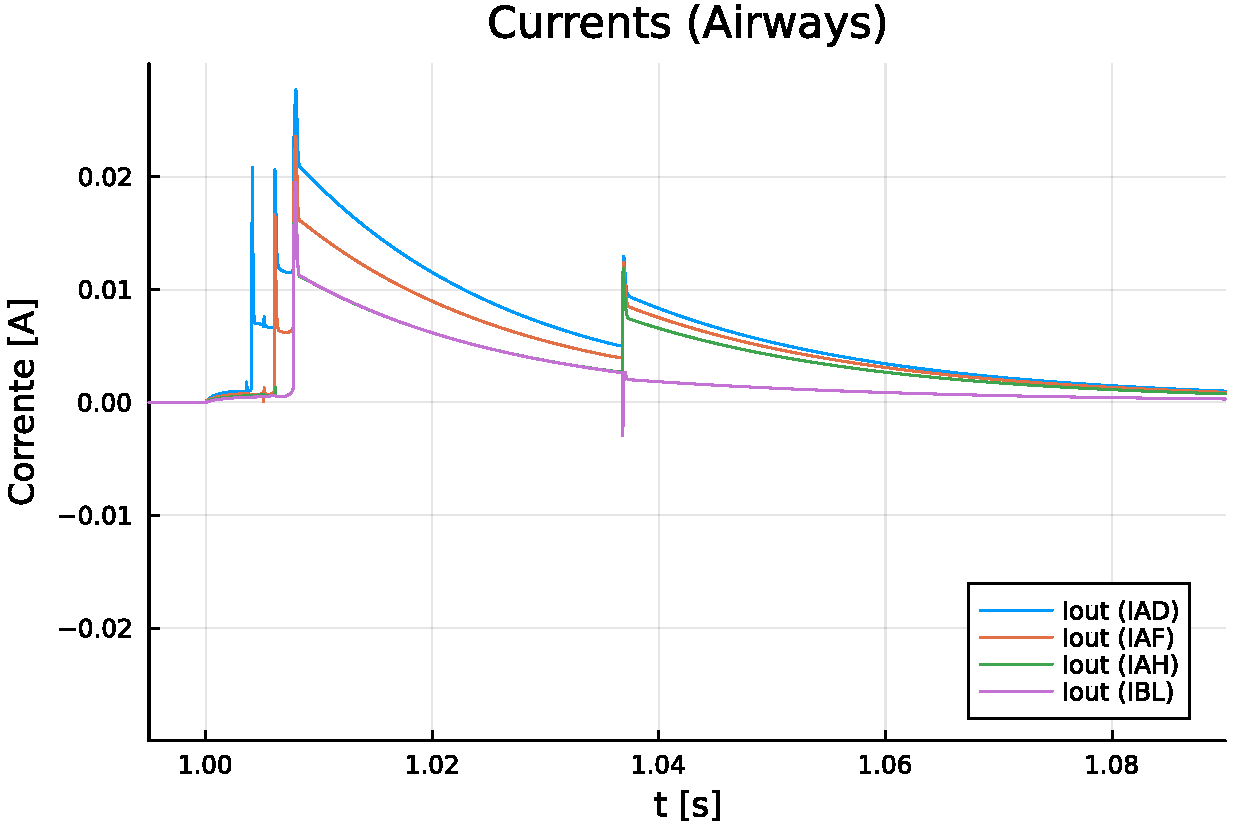
\includegraphics[width=.45\textwidth]{airways_currents_10.pdf}}\\
  \subfloat[][Acini voltages]{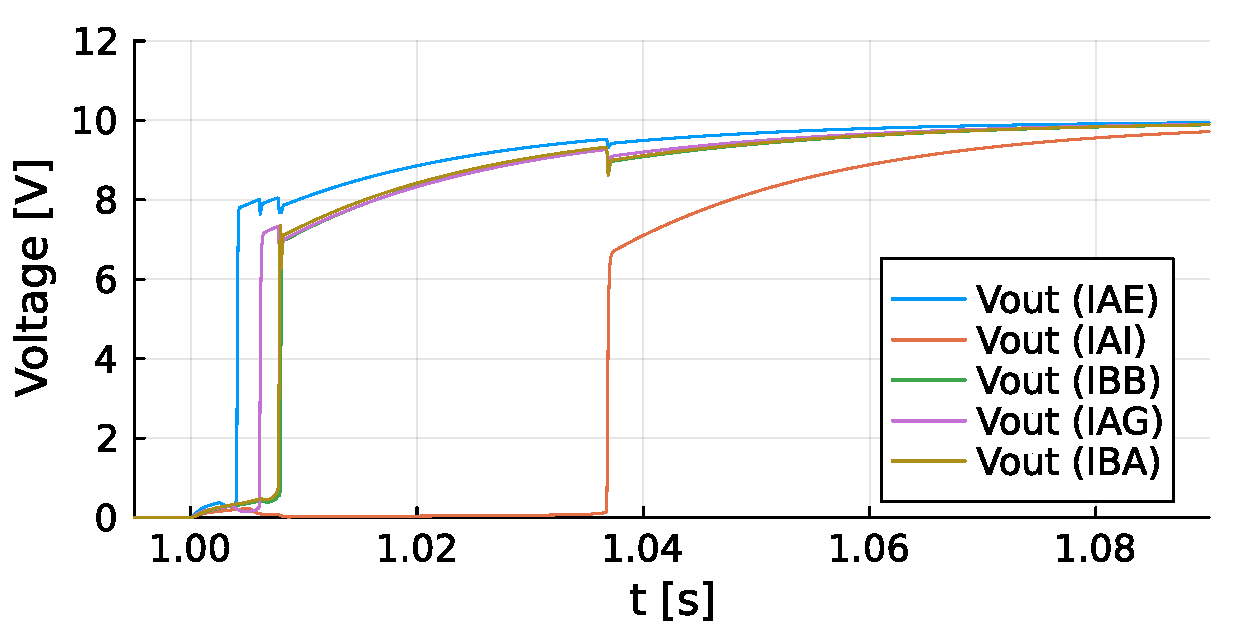
\includegraphics[width=.45\textwidth]{acini_voltages_10.pdf}}%
  \hspace{1cm}
  \subfloat[][Acini currents]{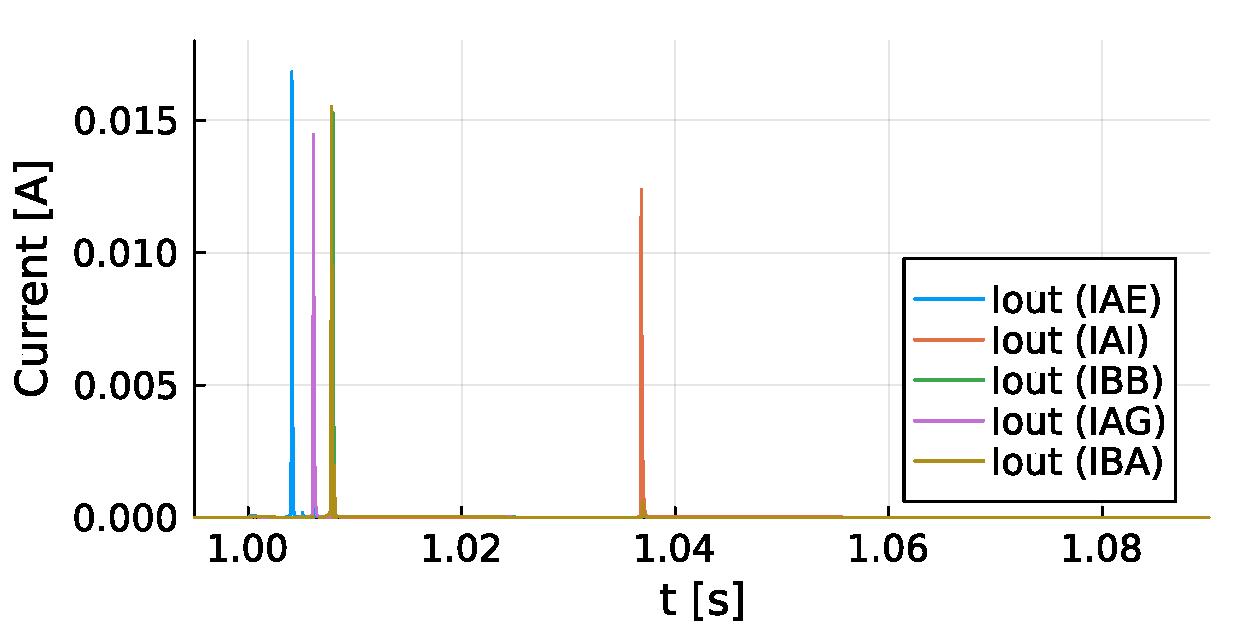
\includegraphics[width=.45\textwidth]{acini_currents_10.pdf}}
  \caption{(Electrically equivalent) mechanical simulation for acini
    and airways.  The step amplitude is 10V.}
  \label{fig:mechanical_results_10_2}
\end{figure}

% Test 1
%% Airways
\begin{table}[H]
  \centering
  \begin{minipage}[h]{.25\textwidth}\centering
    \begin{figure}[H]\centering
  \begin{tikzpicture}[node distance=1.5cm]
    \node (GEN) [rectangle, rounded corners, minimum width=1.5cm, minimum height=.75cm, draw=black, fill=green!25] {Step (10V)};
    \node (IAD) [airway_vertical, below of=GEN]                                                                    {1$^\circ$};
    \node (IAF) [airway_vertical, below of=IAD]                                                                    {2$^\circ$};
    \node (IAH) [airway_vertical, below of=IAF]                                                                    {4$^\circ$};
    \node (IBL) [airway_vertical, below of=IAH]                                                                    {5$^\circ$};
    \node (IAE) [acinus_vertical, left of=IAD, xshift=-.25cm, yshift=-1.5cm]                                       {3$^\circ$};
    \node (IAG) [acinus_vertical, right of=IAF, xshift=.25cm, yshift=-1.5cm]                                       {6$^\circ$};
    \node (IAI) [acinus_vertical, left of=IAH, xshift=-.25cm, yshift=-1.5cm]                                       {9$^\circ$};
    \node (IBA) [acinus_vertical, right of=IBL, xshift=.25cm, yshift=-1.5cm]                                       {7$^\circ$};
    \node (IBB) [acinus_vertical, left of=IBL, xshift=-.25cm, yshift=-1.5cm]                                       {8$^\circ$};

    \draw [arrow1] (GEN) -- (IAD);
    \draw [arrow1] (IAD) -- (IAF);
    \draw [arrow1] (IAF) -- (IAH);
    \draw [arrow1] (IAH) -- (IBL);
    \draw [arrow1] (IAD) -- (IAE);
    \draw [arrow1] (IAF) -- (IAG);
    \draw [arrow1] (IAH) -- (IAI);
    \draw [arrow1] (IBL) -- (IBA);
    \draw [arrow1] (IBL) -- (IBB);
  \end{tikzpicture}
  % \caption{The simulated subtree. Airways are represented in red,
    % acini in yellow.}
  \label{fig:subtree_development_10}
\end{figure}

%%% Local Variables:
%%% mode: LaTeX
%%% TeX-master: "../Thesis"
%%% End:

  \end{minipage}\hspace{1.5cm}
  \begin{minipage}[h]{.6\textwidth}
    {\renewcommand{\arraystretch}{1.2}
      \begin{tabularx}{\textwidth}{|P{6em}|C|C|C|C|}
        \hline
        \rowcolor{red!40}
        \textsc{Airways}
        & IAD
        & IAF
        & IAH
        & IBL\\
        \hline
        \rowcolor{yellow!40}$V_{\text{in,th}}$ [V]
        & 4.67
        & 4.99
        & 5.29
        & 5.59\\
        \hline
        \rowcolor{yellow!40}$T_{\text{open}}$ [s]
        & 1.00246
        & 1.00356
        & 1.00501
        & 1.00611\\
        \hline
        \rowcolor{orange!40}Activ. order
        & 1$^{\circ}$
        & 2$^{\circ}$
        & 4$^{\circ}$
        & 5$^{\circ}$\\
        \hline
      \end{tabularx}
    }
    \caption{Airways opening times and orders when test \#1 is
      performed.}
    \label{tab:airways_test1}
    \vspace{.9cm}
    
    {\renewcommand{\arraystretch}{1.2}
      \begin{tabularx}{\textwidth}{|P{6em}|C|C|C|C|C|}
        \hline
        \rowcolor{blue!25}
        \textsc{Acini}
        & IAE
        & IAG
        & IAI
        & IBA
        & IBB\\
        \hline
        \rowcolor{yellow!40}$V_{\text{in,th}}$ [V]
        & 7.96
        & 8.69
        & 9.25
        & 6.79
        & 7.01\\
        \hline
        \rowcolor{yellow!40}$T_{\text{open}}$ [s]
        & 1.0041
        & 1.0062
        & 1.0369
        & 1.0078
        & 1.0080\\
        \hline
        \rowcolor{orange!40}Activ. order
        & 3$^{\circ}$
        & 6$^{\circ}$
        & 9$^{\circ}$
        & 7$^{\circ}$
        & 8$^{\circ}$\\
        \hline
      \end{tabularx}
    }
    \caption{Acini opening times and orders when test \#1 is
      performed.}
    \label{tab:acini_test1}
  \end{minipage}
  \captionof{figure}{Results summary for test \#1.  On the left, the
    subtree morphology containing the opening order of each module.
    On the right, \Cref{tab:airways_test1,tab:acini_test1} display
    diode thresholds and opening times.}
  \label{fig:mechanical_results_10_1}
\end{table}

% %% Acini
% \begin{table}[H]\centering
%   {\renewcommand{\arraystretch}{1.2}
%     \begin{tabularx}{\textwidth}{|P{6em}|C|C|C|C|C|}
%       \hline
%       \rowcolor{bluePoli!40}
%       \textsc{Acini}
%       & IAE
%       & IAG
%       & IAI
%       & IBA
%       & IBB\\
%       \hline
%       \rowcolor{yellow!40}$V_{\text{in,th}}$ [V]
%       & 7.96
%       & 8.69
%       & 9.25
%       & 6.79
%       & 7.01\\
%       \hline
%       \rowcolor{yellow!40}$T_{\text{open}}$ [s]
%       & 1.00411
%       & 1.00616
%       & 1.03686
%       & 1.00781
%       & 1.00796\\
%       \hline
%       \rowcolor{orange!40}Activ. order
%       & 3$^{\circ}$
%       & 6$^{\circ}$
%       & 9$^{\circ}$
%       & 7$^{\circ}$
%       & 8$^{\circ}$\\
%       \hline
%     \end{tabularx}
%   }
%   \caption{Acini opening times values and total activation order
%     when test \#1 is performed.}
%   \label{tab:acini_test1}
% \end{table}

\clearpage
The second test provides a voltage capable of opening some modules
constituting the subtree.  Opening times and activation orders are
summarized into \Cref{tab:airways_test2,tab:acini_test2}.  Relative
airway activation order is increasing from proximal to distal.  Only
distal acini are activated due to their lower diode thresholds, the
rest remain closed.
\vspace{1.05em}

\begin{figure}[H]\centering
  \subfloat[][Airways voltages]{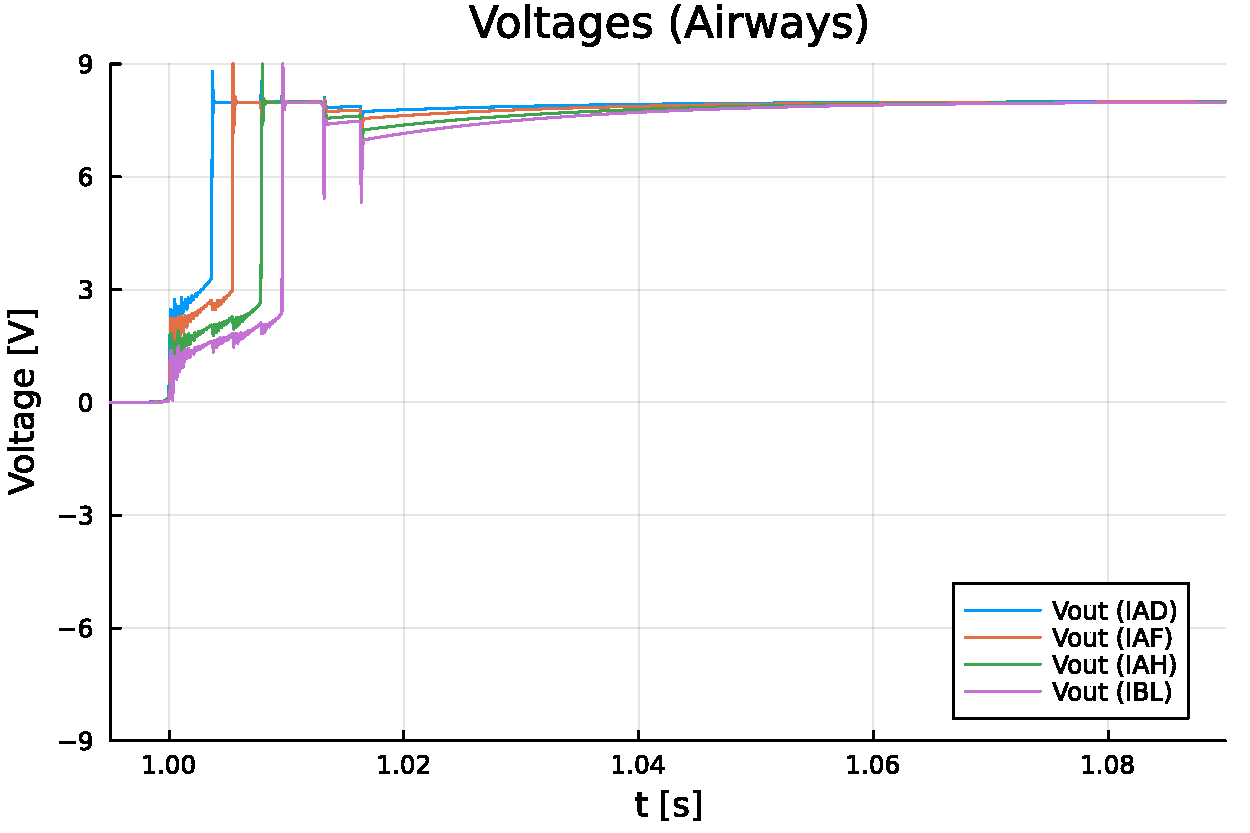
\includegraphics[width=.45\textwidth]{airways_voltages_8.pdf}}%
  \hspace{1cm}
  \subfloat[][Airways currents]{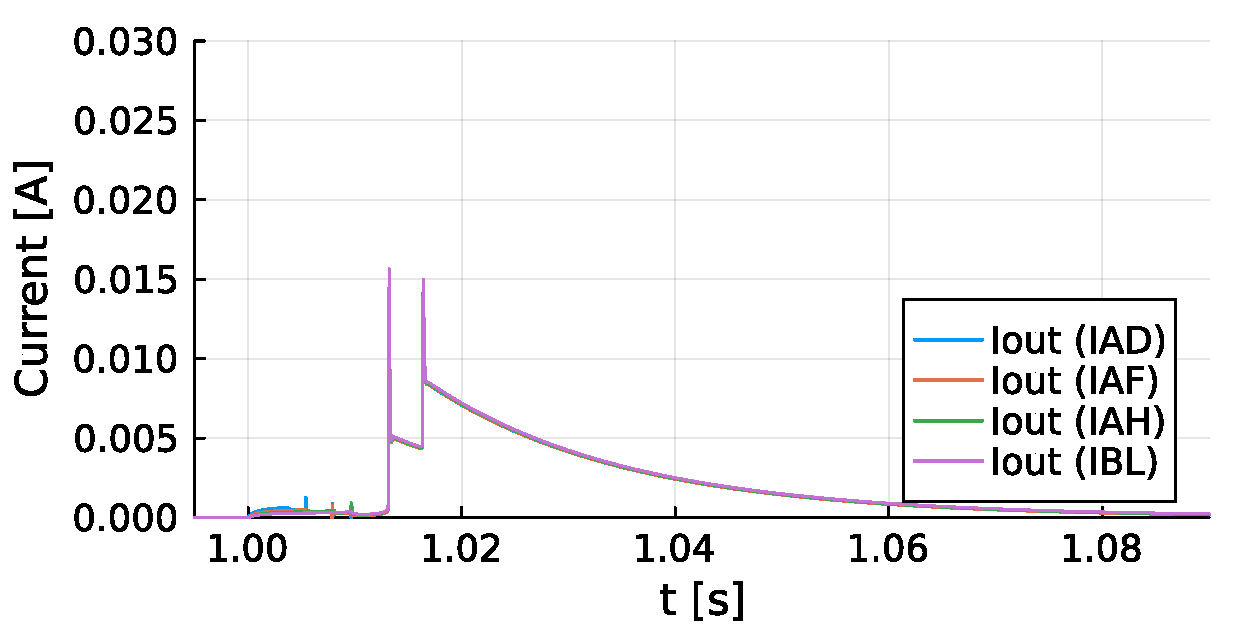
\includegraphics[width=.45\textwidth]{airways_currents_8.pdf}}\\
  \subfloat[][Acini voltages]{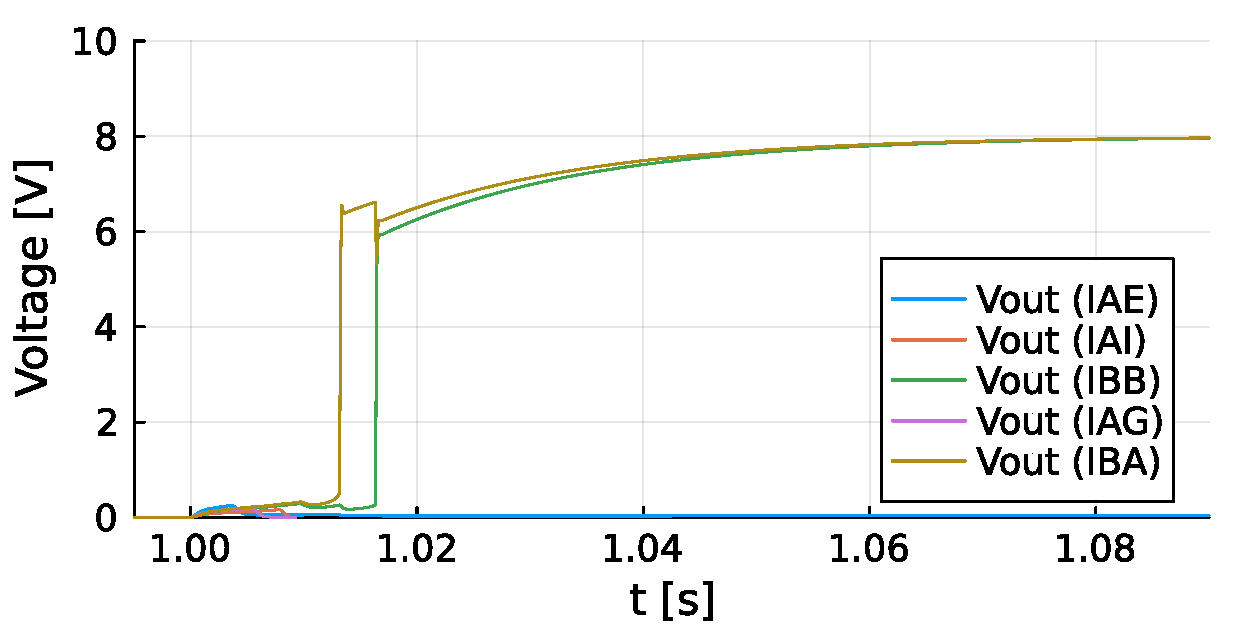
\includegraphics[width=.45\textwidth]{acini_voltages_8.pdf}}%
  \hspace{1cm}
  \subfloat[][Acini currents]{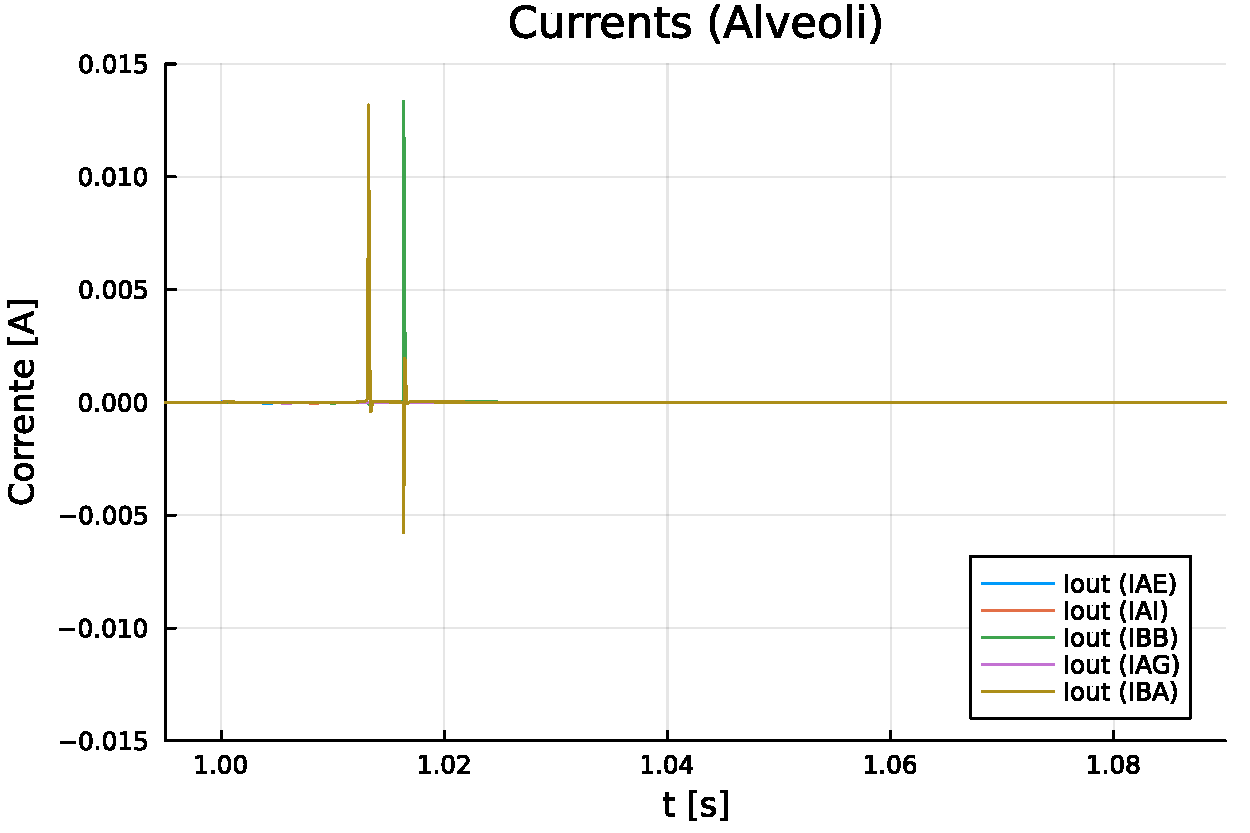
\includegraphics[width=.45\textwidth]{acini_currents_8.pdf}}
  \caption{(Electrically equivalent) mechanical simulation for acini
    and airways.  The step amplitude is 8V.}
  \label{fig:mechanical_results_8_2}
\end{figure}

% Test 2
%% Airways
\begin{table}[H]\centering
  \begin{minipage}{.25\textwidth}\centering
    \begin{figure}[H]\centering
  \begin{tikzpicture}[node distance=1.5cm]
    \node (GEN) [rectangle, rounded corners, minimum width=1.5cm, minimum height=.75cm, draw=black, fill=green!25] {Step (8V)};
    \node (IAD) [airway_vertical, below of=GEN]                                                                    {1$^\circ$};
    \node (IAF) [airway_vertical, below of=IAD]                                                                    {2$^\circ$};
    \node (IAH) [airway_vertical, below of=IAF]                                                                    {3$^\circ$};
    \node (IBL) [airway_vertical, below of=IAH]                                                                    {4$^\circ$};
    \node (IAE) [acinus_vertical, left of=IAD, xshift=-.25cm, yshift=-1.5cm]                                       {---};
    \node (IAG) [acinus_vertical, right of=IAF, xshift=.25cm, yshift=-1.5cm]                                       {---};
    \node (IAI) [acinus_vertical, left of=IAH, xshift=-.25cm, yshift=-1.5cm]                                       {---};
    \node (IBA) [acinus_vertical, right of=IBL, xshift=.25cm, yshift=-1.5cm]                                       {5$^\circ$};
    \node (IBB) [acinus_vertical, left of=IBL, xshift=-.25cm, yshift=-1.5cm]                                       {6$^\circ$};

    \draw [arrow1] (GEN) -- (IAD);
    \draw [arrow1] (IAD) -- (IAF);
    \draw [arrow1] (IAF) -- (IAH);
    \draw [arrow1] (IAH) -- (IBL);
    \draw [arrow1] (IAD) -- (IAE);
    \draw [arrow1] (IAF) -- (IAG);
    \draw [arrow1] (IAH) -- (IAI);
    \draw [arrow1] (IBL) -- (IBA);
    \draw [arrow1] (IBL) -- (IBB);
  \end{tikzpicture}
  % \caption{The simulated subtree. Airways are represented in red,
    % acini in yellow.}
  \label{fig:subtree_8_development}
\end{figure}

%%% Local Variables:
%%% mode: LaTeX
%%% TeX-master: "../Thesis"
%%% End:

  \end{minipage}\hspace{1.5cm}
    \begin{minipage}{.6\textwidth}\centering
    {\renewcommand{\arraystretch}{1.2}
      \begin{tabularx}{\textwidth}{|P{6em}|C|C|C|C|}
        \hline
        \rowcolor{red!40}
        \textsc{Airways}
        & IAD
        & IAF
        & IAH
        & IBL\\
        \hline
        \rowcolor{yellow!40}$V_{\text{in,th}}$ [V]
        & 4.67
        & 4.99
        & 5.29
        & 5.59\\
        \hline
        \rowcolor{yellow!40}$T_{\text{open}}$ [s]
        & 1.00361
        & 1.00536
        & 1.00781
        & 1.00961\\
        \hline
        \rowcolor{orange!40}Activ. order
        & 1$^{\circ}$
        & 2$^{\circ}$
        & 3$^{\circ}$
        & 4$^{\circ}$\\
        \hline
      \end{tabularx}
    }
    \caption{Airways opening times and orders when test \#2 is
      performed.}
    \label{tab:airways_test2}
    \vspace{.9cm}
    {\renewcommand{\arraystretch}{1.2}
      \begin{tabularx}{\textwidth}{|P{6em}|C|C|C|C|C|}
        \hline
        \rowcolor{blue!25}
        \textsc{Acini}
        & IAE
        & IAG
        & IAI
        & IBA
        & IBB\\
        \hline
        \rowcolor{yellow!40}$V_{\text{in,th}}$ [V]
        & 7.96
        & 8.69
        & 9.25
        & 6.79
        & 7.01\\
        \hline
        \rowcolor{yellow!40}$T_{\text{open}}$ [s]
        & $+\infty$
        & $+\infty$
        & $+\infty$
        & 1.01316
        & 1.01636\\
        \hline
        \rowcolor{orange!40}Activ. order
        & ---
        & ---
        & ---
        & 5$^{\circ}$
        & 6$^{\circ}$\\
        \hline
      \end{tabularx}
      \caption{Acini opening times values and total activation order
        when test \#2 is performed.}
      \label{tab:acini_test2}
    }
  \end{minipage}
  \captionof{figure}{Results summary for test \#2.  On the left, the
    subtree morphology containing the opening order of each module.
    On the right, \Cref{tab:airways_test2,tab:acini_test2} display
    diode thresholds and opening times. Long dashes: no opening has
    occurred.}
  \label{fig:mechanical_results_8_1}
\end{table}

% %% Acini
% \begin{table}[H]\centering
% \end{table}

%%% Local Variables:
%%% mode: LaTeX
%%% TeX-master: "../Thesis"
%%% End:
